% Routing map (Stage 3). Region boundaries follow the dispatch rules of
% tab:dispatch-rules: Tier 1 iff 0.70 s + 0.30 u >= 0.90; else Tier 2 iff s >= 0.75.
\begin{figure}[!htbp]
\centering
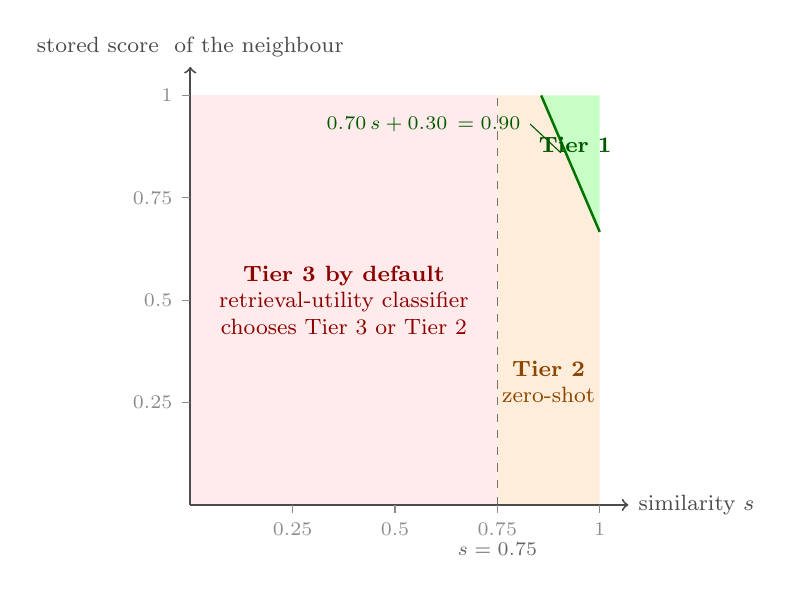
\begin{tikzpicture}[scale=5.2, font=\small]
  \fill[red!8]   (0,0) rectangle (0.75,1);
  \fill[orange!14] (0.75,0) -- (1,0) -- (1,0.6667) -- (0.857,1) -- (0.75,1) -- cycle;
  \fill[green!22] (0.857,1) -- (1,1) -- (1,0.6667) -- cycle;
  \draw[dashed, black!55, line width=0.6pt] (0.75,0) -- (0.75,1);
  \draw[green!45!black, line width=0.9pt] (0.857,1) -- (1,0.6667);
  \draw[->, black!70, line width=0.7pt] (0,0) -- (1.07,0) node[right, font=\footnotesize] {similarity $s$};
  \draw[->, black!70, line width=0.7pt] (0,0) -- (0,1.07) node[above, font=\footnotesize] {stored score $\ustored$ of the neighbour};
  \foreach \x in {0.25,0.5,0.75,1} \draw[black!45] (\x,0) -- (\x,-0.02) node[below, font=\scriptsize] {\x};
  \foreach \y in {0.25,0.5,0.75,1} \draw[black!45] (0,\y) -- (-0.02,\y) node[left, font=\scriptsize] {\y};
  \node[align=center, text=red!55!black, font=\footnotesize] at (0.375,0.5) {\textbf{Tier 3 by default}\\retrieval-utility classifier\\chooses Tier 3 or Tier 2};
  \node[align=center, text=orange!55!black, font=\footnotesize] at (0.875,0.3) {\textbf{Tier 2}\\zero-shot};
  \node[text=green!35!black, font=\footnotesize\bfseries] at (0.94,0.88) {Tier 1};
  \node[anchor=east, font=\scriptsize, text=green!35!black] at (0.83,0.93) {$0.70\,s + 0.30\,\ustored = 0.90$};
  \draw[green!35!black, line width=0.4pt] (0.83,0.93) -- (0.905,0.86);
  \node[anchor=north, font=\scriptsize, text=black!60] at (0.75,-0.07) {$s = 0.75$};
\end{tikzpicture}
\caption[Routing map of the three-tier router.]{Routing map of the three-tier router. Before this map is consulted, the safety override sends any query with $\upre < 0.38$ to the retrieval-utility classifier.}
\label{fig:routing-map}
\end{figure}
